\documentclass[conference]{IEEEtran}
\IEEEoverridecommandlockouts
\usepackage{cite}
\usepackage{amsmath,amssymb,amsfonts}
\usepackage{algorithmic}
\usepackage{graphicx}
\usepackage{textcomp}
\usepackage{xcolor}

\usepackage{url}
\def\UrlFont{\rmfamily}

\usepackage{pgf-pie}

\usepackage{caption}


\def\BibTeX{{\rm B\kern-.05em{\sc i\kern-.025em b}\kern-.08em
    T\kern-.1667em\lower.7ex\hbox{E}\kern-.125emX}}
\begin{document}

\title{Exploring the Vulnerabilities of IoT Devices: A Comprehensive Analysis of Mirai and Bashlite Attack Vectors}

\author{
\IEEEauthorblockN{Seth Barrett, Bradley Boswell,  and Gokila Dorai}
\IEEEauthorblockA{\textit{School of Computer and Cyber Sciences, Augusta University}\
Augusta, USA\ 
\\ \{sebarrett, brboswell, gdorai\}@augusta.edu}
}

\maketitle

\begin{abstract}
Our paper provides crucial insights into IoT device security, emphasizing the need for risk mitigation on the edge. This research not only raises security awareness among manufacturers, developers, and end-users, but also guides the development of better defense mechanisms and security protocols for IoT devices, including edge computing environments. The findings can influence policy and regulation, leading to the creation of security guidelines and standards for IoT manufacturers, ensuring robust protection even at the network periphery. This research fosters a safer environment for IoT growth in various sectors, educates users on potential risks and steps to secure their devices, and underscores the importance of edge security. Moreover, the study stimulates further research in the field, advancing the collective understanding of attack vectors and development of novel security solutions that cater to the unique challenges of edge computing.
\end{abstract}

\begin{IEEEkeywords}
Internet of Things (IoT), IoT Device Security, Edge Computing, Security Protocols, Attack Vectors
\end{IEEEkeywords}

\section{Introduction}

The rapid proliferation of the Internet of Things (IoT) has resulted in an unprecedented interconnection of devices across various spheres of modern life. IoT has seen an extensive application range, from enhancing comfort and efficiency in homes through automation to streamlining industrial processes and bolstering productivity. However, the attributes contributing to the IoT's widespread adoption—interconnectivity and remote accessibility—also serve as a double-edged sword, potentially exposing these devices and their networks to a broad range of cyber threats \cite{9800047}.

Mainly, IoT devices often constitute the edge of a network. Therefore, robust security measures must be implemented at this level to amplify the need for these devices to become a crucial line of defense against potential threats. As the number of IoT devices grows, the associated attack surface expands correspondingly, engendering a pressing need to address concerns about device security and data integrity \cite{DBLP:journals/corr/abs-2003-01218}. Considering notorious threats such as the Bashlite and Mirai botnets, which have exploited vulnerabilities in IoT devices, it is especially critical to emphasize security \cite{DBLP:journals/corr/abs-2104-09041,bertino2017botnets}.
In our research, we thoroughly examine various IoT devices within a network context. We systematically identify and scrutinize vulnerabilities commonly exploited by the aforementioned botnets. This exploration is of great importance to understand the landscape of real-world attacks on IoT devices and provide insights for improving the security posture of these devices \cite{DBLP:journals/corr/abs-2003-01218}.

Our research underscores the urgent need for comprehensive risk mitigation strategies at the network edge, illuminating the security implications for device manufacturers, software developers, and end-users. Our study also contributes to developing improved defense mechanisms and security protocols, particularly tailored to address the unique challenges presented by edge computing environments \cite{abomhara2015cyber}.

Significantly, our research extends beyond technical countermeasures. The findings from this study serve to inform policy decisions and regulatory measures, underscoring the role of governance in fostering a secure IoT environment. In this context, our investigation shapes the development of stringent security guidelines and standards to which IoT device manufacturers should adhere. These standards are expected to ensure robust protection, even at the network periphery, thereby safeguarding data integrity and system stability \cite{8490192,vignau201910}.

Overall, our paper aims to facilitate the creation of a safer environment that would enable IoT's continued growth and evolution across various sectors. It also aims to educate users on potential risks associated with IoT devices and the steps they can take to secure them, underscoring the importance of security awareness and education in the IoT domain \cite{8490192}. 

Our findings contribute to the broader collective understanding of attack vectors and their mitigation. Furthermore, this research contributes to the development of novel security solutions that cater to the unique security challenges posed by IoT devices and edge computing \cite{DBLP:journals/corr/abs-2104-09041}. Specifically, the primary contributions of our work are:
\begin{itemize}
\item Detailed analysis of IoT device vulnerabilities: Through meticulous experimental design, we have unveiled critical insights related to the network behaviors of popular IoT devices in flooding scenarios (UDP, HTTP, TCP, XMAS). We found that less than 50\% of the devices in our controlled lab environment had vulnerabilities with respect to our four flooding attacks.
\item Emphasizing the role of edge computing in IoT security: Our research underscores the security risks posed by the shift to edge computing, highlighting an important and often overlooked aspect of IoT security.
\item Real-world relevance: The findings from our research have significant real-world implications. They provide a roadmap for improving the security of IoT devices in actual network environments, contributing to safer and more reliable IoT ecosystems.
\end{itemize}

\begin{table}[]
\caption{Comparison of contributions}
\begin{tabular}{p{4cm}p{1.5cm}p{2cm}}
\hline
Contributions & Our Work & Other Papers \\ \hline
    Detailed analysis of IoT device vulnerabilities & Yes  & Partially \cite{williams2017identifying,butun2019security} \\ %\hline
    
    Role of edge computing in IoT security & Yes  & No \cite{8490192,9090824,williams2017identifying,butun2019security,ahamed2016internet} \\ %\hline
    
    Comprehensive dataset generation & Yes  & Partially \cite{williams2017identifying} \\ %\hline
    
    Development of robust security measures & Yes  & Partially \cite{8490192,9090824} \\ %\hline
    
    Risk mitigation strategies at the network edge & Yes  & Yes \cite{9090824} \\ %\hline
    
    Improved defense mechanisms and security protocols & Yes  & Partially \cite{8490192,9090824} \\ %\hline
    
    Comprehensive understanding of IoT device security & Yes  & Partially \cite{butun2019security} \\ %\hline
    
    Testing vulnerabilities frequently targeted by botnets & Yes  & No \cite{8490192,9090824,williams2017identifying,butun2019security,ahamed2016internet} \\ %\hline
    
    Application of Machine Learning techniques in IoT security & Yes  & Yes \cite{8490192} \\ \hline
\end{tabular}
\label{tab:contributions}
\end{table}


By systematically examining the vulnerabilities of IoT devices under various attack scenarios in a controlled environment, this research contributes to the development of more robust, effective, and context-specific security measures, ultimately fostering a more secure IoT ecosystem in the face of evolving cyber threats.

\section{Background and Related Work}
 The Internet of Things (IoT) revolution has yielded a boom of interconnected devices across the Internet, offering benefits such as efficient resource utilization, automation, and real-time monitoring \cite{butun2019security}. Despite these benefits, the concurrent surge in security vulnerabilities presented by these devices has rendered them susceptible to cyber-attacks, leading to a vital shift of research focus towards IoT security challenges \cite{DBLP:journals/corr/abs-2003-01218,williams2017identifying,8796409}.

The diverse spectrum of IoT devices provides a broad canvas for malicious actors, giving rise to various attacks \cite{neshenko2019demystifying}. Among these, Distributed Denial of Service (DDoS) attacks have been extensively examined \cite{DBLP:journals/corr/abs-2104-09041}, \cite{9090824}. Numerous studies, including the work of Moody and Hunter, have explored how known vulnerabilities in IoT devices, such as smart thermostats, can be exploited \cite{moody2016exploiting}.

Building on the insightful work of Tabari and Ou \cite{DBLP:journals/corr/abs-2003-01218} and Meneghello et al. \cite{8796409}, which brought to light the actuality of attacks on IoT devices and provided insights into these attacks' landscapes, we aim to understand further and test the practical vulnerabilities that attackers exploit.

Notably, the emergence of botnets targeting IoT devices, thereby transforming the Internet of Things into an Internet of Vulnerabilities (IoV), has been a crucial watershed in the research community \cite{angrishi2017turning}. Meidan et al.'s work \cite{8490192} has significantly advanced the understanding of botnet attacks on IoT networks, culminating in a network-based detection method using deep autoencoders, paving the way for anomaly detection and bolstering IoT device security.

The exploration by Tushir et al. \cite{DBLP:journals/corr/abs-2104-09041} into the effects of DoS attacks on resource-constrained IoT devices, with an emphasis on the Mirai attack, along with Özalp et al.'s in-depth study of the multiple layers of IoT cyber-attacks \cite{9800047}, underscore the urgent need for effective countermeasures against such attacks.

Ferrara et al.'s work \cite{ferrara2021static} shows promise in using static analysis to uncover IoT vulnerabilities, suggesting a promising direction for enhancing IoT device security.

Our research contributes to this existing corpus of knowledge by focusing on delivering a more comprehensive understanding of IoT device security, specifically in the context of edge computing environments (see Table \ref{tab:contributions}). Our unique approach involves testing vulnerabilities frequently targeted by botnets such as Bashlite and Mirai across a range of IoT devices, bridging gaps in understanding and offering new perspectives on IoT device security. Further, we aim to harness the power of Machine Learning (ML) techniques to detect and mitigate these vulnerabilities, thus pioneering a significant advancement in IoT and ML security research.

% 
\section{Problem Statement}

The emergence and proliferation of Internet of Things (IoT) devices have unfolded numerous possibilities for innovation, automation, and optimization across a broad range of sectors \cite{butun2019security}. However, the expansion of this IoT ecosystem unavoidably presents an escalating spectrum of security vulnerabilities. The surge of edge computing, a computing paradigm that pushes data processing to the network's periphery, further exacerbates these risks \cite{angrishi2017turning}.

\begin{itemize}
\item The problem at the heart of these challenges is the unique nature of IoT devices, their diversity, and the sheer number of entry points, which offer a vast surface area for cyber adversaries \cite{neshenko2019demystifying}. These issues are further magnified in resource-constrained edge computing environments \cite{DBLP:journals/corr/abs-2104-09041}. Traditional security solutions often falter due to many IoT devices' inherent computational and power limitations, necessitating innovative, custom-fit security solutions designed explicitly for IoT devices operating within edge computing environments.

\item One of the most profound threats looming over IoT devices today is the risk of botnets, which can severely undermine the functionality of these devices and use them as launchpads for coordinated cyber-attacks \cite{8490192}. The Mirai attack serves as a stark reminder of how botnets can commandeer IoT devices to orchestrate extensive Distributed Denial of Service (DDoS) attacks, underscoring the need for bolstered security measures \cite{DBLP:journals/corr/abs-2104-09041}. This brings us to a central problem: the need for advanced detection and defense strategies to mitigate botnet attacks, specifically within edge computing environments effectively \cite{9800047}.

\item Moreover, IoT devices harbor various vulnerabilities ripe for exploitation by malicious actors \cite{8796409}. Many of these weaknesses stem from known software flaws, underscored by Moody and Hunter's exploration of smart thermostats \cite{moody2016exploiting}. Such vulnerabilities emphasize the necessity for more rigorous vulnerability testing and remediation strategies.

\item While promising, emerging methodologies like static analysis are still in their infancy and often grapple with effectively identifying and addressing IoT vulnerabilities \cite{ferrara2021static}. This predicament underscores a critical gap: the absence of efficient and reliable tools for vulnerability detection in IoT devices, which necessitates the development of innovative detection methods.
\end{itemize}

Thus, a central problem this research aims to tackle is: How can we leverage machine learning to design an effective Intrusion Detection and Prevention System (IDPS) specifically optimized for IoT devices in edge computing environments? Another critical question arises: How can we generate and share open-source datasets of IoT attack packets and baseline data that can be leveraged to train and evaluate these IDPS models \cite{lakshmanan2020literature}?

To address these questions, our study strives to enhance our understanding of IoT device security, particularly within the edge computing environment. We aim to examine the vulnerabilities botnets exploit across a diverse set of IoT devices and create an open-source dataset of baseline and attack packet data. This dataset will provide the groundwork for developing an edge-optimized ML IDPS model, thus enhancing IoT device security in consumer and enterprise environments. Ultimately, our research findings could lead to significant real-world implications, including more secure and resilient IoT ecosystems.

% 
\section{Methodology}
In our study, we utilized a comprehensive and rigorous methodology to elucidate the nature of vulnerabilities in IoT devices and their behavior under various attack scenarios. We characterize our approach through meticulous experimental design and robust data collection protocols, mirroring real-world network environments and interactions. We organize this methodology into three stages: 1) setting up the test environment, 2) capturing and analyzing non-attack packets and interactions, and 3) capturing packets under attack conditions. By constructing a faithful replication of actual network conditions, we aimed to facilitate a profound understanding of IoT device vulnerabilities and provide a foundation for robust security solutions \cite{DBLP:journals/corr/abs-2104-09041,DBLP:journals/corr/abs-2003-01218}. 


\subsection{Test Environment Set-Up}

In order to rigorously investigate the security vulnerabilities of IoT devices, we needed to emulate a real-world network environment where these devices typically operate. To this end, we established a secure, controlled network environment in our lab. Fig. \ref{fig:device_pics_label} shows the centerpiece of this network was a TP-Link TL-WR541N router running the open-source OpenWrt firmware. The choice of this router model and firmware was motivated by several factors. Firstly, OpenWrt's flexibility and extensibility allowed us to gain granular control over the network settings. Secondly, this router supports dual-bandwidth operation (2.4GHz and 5GHz), an essential feature given the diversity of IoT devices we intended to test \cite{DBLP:journals/corr/abs-2003-01218}. 

We conducted initial experiments using a single-band (5GHz) router. However, we quickly realized that several IoT devices, particularly those designed for household use, exclusively operated on the 2.4GHz band. Therefore, we upgraded to a dual-band router to ensure compatibility with all our test devices.

% Confirm updates are solid
\begin{figure}[t]
\centering
\fbox{
\includegraphics[width=0.475\textwidth]{Network3Gray.png}}
\caption{Experimental Setup}
\label{fig:device_pics_label}
\end{figure}

We selected a range of IoT devices for testing, representing various categories and usage contexts. The range of IoT devices, representing various categories and usage contexts, is generally sufficient to draw some conclusions for scientific purposes. These included a 4th Generation Amazon Echo Dot, Kasa Smart Plug, LongPlus Smart PTZ Camera, 2nd Generation Ring Doorbell, Google Nest/Home Mini, Google Home Cam, and NiteBird Smart LED Light Bulb as seen in Table \ref{tab:testenv}. Each device was connected to the router and fully set up using their respective companion apps on a Samsung Galaxy A71 5G smartphone. We guided the device selection based on previous works that showcased the diversity of IoT devices and their varying degrees of vulnerability to different types of attacks \cite{DBLP:journals/corr/abs-2104-09041,8490192}. 


We acquired some devices but have not included them in the initial pool. These included a Level Lock, Level Keypad, and FitBit Charge 4, which only supported Bluetooth connectivity. We also excluded the Nest Learning Thermostat because it requires a connection to a physical HVAC system, which we intend to emulate in future work.

We used Wireshark on a Windows laptop during the preliminary phase to capture network packets from the devices for initial analysis. We quickly realized that the devices frequently changed their local IP addresses, potentially complicating our data collection process. As such, we assigned static IP addresses to each device to prevent IP changes during our experiments. 

\begin{table}[t]
\small
  \centering
  \caption{Test Environment}
  \begin{tabular}{lp{5cm}l}
     \hline
     Item & Description \\
     \hline
     IoT Devices & (1) Amazon Echo Dot, 5\textsuperscript{th} Generation (Model Number: B7W644)\cite{dot}, (Quantity: 1) \\
     	&	(2) Kasa Smart Wi-Fi Plug Mini (Model Number: HS105)\cite{kasa}, (Quantity: 1)\\
     	&	(3) LongPlus Baby Monitor (Model Number: X07)\cite{longplus}, (Quantity: 1)	\\
        &	(4) Ring Video Doorbell, 2\textsuperscript{nd} Generation\cite{ring}, (Quantity: 1)\\
        &	(5) Google Nest Mini (Model Number: H2C)\cite{nestMini}, (Quantity: 1) \\
        &	(6) Google Nest Cam (indoor, wired) (Model Number: GJQ9T)\cite{nestcam}, (Quantity: 1) \\
        &	(7) NiteBird Smart Bulb (Model Number: WB4-2-US)\cite{nitebird} (Quantity: 1) \\ 
        

        
     Other Devices/Apps & (1) Samsung Galaxy A71 5G (Android 13) \\
     	& 	(2) Acer Aspire A515-56 (Windows 10 v21H2) \\
        &   (3) Amazon Alexa Android App (v2.2.485772.0) \\
     	&	(4) Gosund Android App (v5.1.72) \\
            &	(5) Google Home Android App (v2.60.1.14) \\
            &	(6) LongPlus Android App (v22.1.22.20221031) \\
      	&	(7) Ring Android App (v3.54.1) \\
       &	(8) WireShark Windows App (v4.0.1-0-ge9f3970b1527) \\
       & (9) Hping3 Windows App (v 3.0.0-alpha-1) \\
       & (10) Nmap Windows App (v7.91) \\

        
     Testing period & 2022-08-06 to 2023-05-01 \\
     \hline
	\end{tabular}
    \label{tab:testenv}
\end{table}

\subsection{Non-Attack Packet Capture and Interaction Analysis}

We began by capturing network traffic over periods of both 24 hours and 72 hours with all IoT devices connected and operating normally on the network. The network capture tool of choice was Wireshark, owing to its comprehensive feature set and widespread usage in the network security community \cite{DBLP:journals/corr/abs-2003-01218}. The Windows laptop previously introduced served as the collection point for all packet capture sessions. 

Following this, we disconnected all the devices from the network and conducted separate 24-hour capture sessions for each device. The motivation behind this decision was to isolate the unique communication patterns of each device. We designed these sessions so that the network would comprise only the IoT device under test, the Windows laptop, and our lab's smartphone. 

To ensure we captured a wide range of typical interactions, we engaged with each IoT device using various methods, including physical sensors and accompanying smartphone applications. Table \ref{table:devices_interactions} presents a summary of the interaction methods per device. 

\begin{table}[htbp]
\centering
\caption{IoT Devices and Corresponding Interaction Methods}
\label{table:devices_interactions}
\begin{tabular}{p{0.4\linewidth}p{0.5\linewidth}}
\hline
Device Name & Interaction Methods \\
\hline
Amazon Echo Dot, 5\textsuperscript{th} Generation & Smartphone App and Voice Interaction \\
% \hline
Kasa Smart Wi-Fi Plug Mini & Smartphone App and Physical Button \\
% \hline
LongPlus X07 Baby Monitor & Smartphone App \\
% \hline
Ring Video Doorbell, 2\textsuperscript{nd} Generation & Smartphone App and Device Controller \\
% \hline
Google Nest Mini & Smartphone App and Voice Interaction \\
% \hline
Google Home Cam & Smartphone App \\
% \hline
NiteBird Smart Bulb & Smartphone App \\
% \hline
\end{tabular}
\end{table}

With the captured packet data and the detailed interaction logs, we constructed a comprehensive view of the typical network behavior of these IoT devices. This baseline data would subsequently serve as an invaluable asset in identifying and mitigating IoT device vulnerabilities.

\subsection{Under Attack Scenario - Packet Capture}
\label{sec:method:attackPcap}

As we aimed to understand the behavior of IoT devices under network attacks, our subsequent research stage was to conduct attack packet captures. The strategy was to expose each IoT device to a set of attacks, recording the resulting packet data. These captures provided the insights needed to analyze how the IoT devices responded when under different types of network attacks.\cite{alrawi2019sok}

To maintain control and reliability in our experimentation, we decided to connect only one device to the network during each attack. We started by recording the network traffic for an initial 8-hour period without an attack to serve as a baseline comparison. After this period, we launched a specific attack while recording the packet data, terminating the capture once the attack had ceased. This method allowed us to understand the specific network behaviors associated with each attack on each device. 

Our attack suite comprised a variety of standard and potent network attacks, including a TCP/SYN Flood\cite{eddy2007tcp}, XMAS Tree Flood\cite{xmasFlood}, UDP Flood\cite{udpFlood}, and HTTP Flood\cite{httpFlood}. We aimed to replicate common forms of malicious traffic IoT devices might encounter in real-world settings \cite{DBLP:journals/corr/abs-2104-09041,martin2019raspberry}. 

We employed a Raspberry Pi 3b running Kali Linux to facilitate these attacks. The Pi was an ideal choice due to its versatility, power, and a rich library of penetration testing tools readily available on the Kali platform. We accessed the Raspberry Pi remotely using SSH from the Windows laptop previously mentioned, from which we could initiate our attacks in a controlled manner. 

In order to initiate the different types of attacks, we used specific commands readily available in Kali Linux. The commands used to launch each type of attack are located in Table \ref{tab:attack_launching}.

\begin{table}[htbp]
\centering
\caption{Commands Used for Launching Attacks}
\label{tab:attack_launching}
\begin{tabular}{p{0.4\linewidth}p{0.5\linewidth}}
\hline
Attack Type & Command \\
\hline
XMAS Tree Flood\cite{xmasFlood} on ports 1-100 & \texttt{nmap -sX -p 1-100 [ipAddr]} \\
% \hline
TCP/SYN Flood\cite{eddy2007tcp} on port 443 & \texttt{hping3 -S -c 100 -p 443 [ipAddr]} \\
% \hline
UDP Flood\cite{udpFlood} on port 53 & \texttt{hping3 --udp -c 100 -p 53 [ipAddr]} \\
% \hline
HTTP Flood\cite{httpFlood} & \texttt{hping3 -S -c 100 -p 80  [ipAddr]} \\
\hline
\end{tabular}
\end{table}

As a result, we obtained four attack packet captures for each IoT device, each of which included an 8-hour capture of regular traffic preceding the attack. This strategy provided us with a rich dataset for the following analysis. 

\section{Findings and Discussion}
The results of our investigation have revealed various vulnerabilities across the examined IoT devices, providing an illuminating perspective into their susceptibilities to different types of network attacks \cite{DBLP:journals/corr/abs-2003-01218,DBLP:journals/corr/abs-2104-09041}. We further delve into the analysis, discussing each vulnerability's security implications and potential mitigation strategies. 

\subsection{Device Identifications and Preliminary Scans} 
Our preliminary \texttt{nmap} scans successfully identified all devices under test, facilitating a more in-depth exploration of their network behavior. This identification was crucial for providing a vast landscape of potential security vulnerabilities in each device. The comprehensive scan and a systematic enumeration of services, ports, and other essential information yielded valuable insights into each device's operational behavior and potential vulnerabilities. 

\subsection{TCP and HTTP Flood Attack Vulnerabilities} 
Our experimental results revealed some IoT devices to be particularly susceptible to TCP and HTTP Flood attacks as seem in Fig. \ref{fig:affected_devices}. Specifically, the Kasa Smart Plug demonstrated disruptions in its operation under the TCP Flood attack. Similarly, the LongPlus Smart PTZ Camera and NiteBird Smart LED Light Bulb experienced operational degradation under both TCP and HTTP Flood attacks \cite{DBLP:journals/corr/abs-2104-09041,martin2019raspberry}. The impact of these attacks on device functionality signifies a vulnerability that malicious actors could potentially exploit to disrupt or manipulate device operations. Moreover, the successful launch of these attacks underscores the need for improved defenses against flood attacks in IoT devices. Countermeasures could include rate limiting, traffic shaping, and intrusion detection systems designed to identify and mitigate such attacks \cite{alrawi2019sok}. 

\subsection{Resistance to XMAS and UDP Flood Attacks} 
Contrary to the results from TCP and HTTP Flood attacks, all devices under test remained unaffected by XMAS Tree and UDP Flood attacks. However, it is essential to note that the absence of immediate disruption does not denote the absence of vulnerability. The ability to perform these attacks may provide malicious actors with valuable information about the devices and potentially pave the way for more sophisticated attacks \cite{DBLP:journals/corr/abs-2003-01218,martin2019raspberry}. 

\subsection{Unaffected Devices} 
The Amazon Echo Dot, Ring Doorbell (2nd Generation), Google Nest Mini, and Google Home Cam remained unaffected by all the tested attack types. While these devices demonstrated resilience in our current testing environment, we cannot definitively state that they are impervious to other forms of attack. It is crucial to understand that security is not a static state but a constant endeavor that requires regular testing, patching, and updating to address evolving threats \cite{alrawi2019sok,DBLP:journals/corr/abs-2104-09041}. 


\begin{figure}[t]
\centering
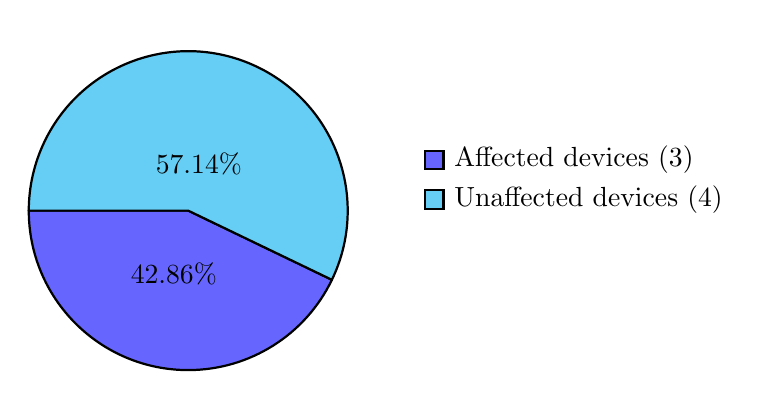
\begin{tikzpicture}[scale=0.675]
    \pie[rotate = 180, text = legend]{
        42.86/Affected devices (3),
        57.14/Unaffected devices (4)
    }
\end{tikzpicture}
\caption{Devices affected by either HTTP Flood or TCP Flood}
\label{fig:affected_devices}
\end{figure}

\subsection{Implications and Future Work} 
The outcomes of this research yield substantial implications, not just within the academic domain but also in real-world scenarios where IoT devices are pervasively deployed. Our findings illuminate the urgency of comprehensive security testing and continual updates to device firmware as defensive measures against an ever-evolving landscape of cyber threats. In addition, the study underscores the need for enhanced user education about potential security vulnerabilities inherent in IoT devices and the proactive steps they can adopt to mitigate these threats.

From a broader perspective, the insights derived from this research can significantly influence the development of future IoT devices. Manufacturers can leverage this knowledge to enhance their product design and security protocols by shedding light on existing vulnerabilities and common attack vectors. This aligns with the global urgency to improve IoT device security and create a more resilient Internet of Things.

Looking towards the future, our research team is eager to delve deeper into the IoT security paradigm. We plan to explore more advanced and complex attack scenarios and assess how IoT devices react under these heightened threats. This future research will allow us to extrapolate further insights into the behavior of IoT devices under varying degrees of cyber threats, enriching our understanding of their vulnerabilities and potential defenses.

In parallel, we aim to investigate the development of intrusion detection and prevention systems uniquely tailored for IoT devices, utilizing the valuable data generated through our research \cite{DBLP:journals/corr/abs-2104-09041}. By leveraging Machine Learning techniques optimized for edge devices, these specialized systems would offer robust and adaptive security solutions that are critically needed to protect IoT devices in consumer and enterprise environments.

In addition, we will make the dataset produced during this research publicly accessible, not only benefiting other researchers and practitioners in the field but also underlining the pragmatic implications of our study. This will include provisions for academic researchers to request access, in an effort to encourage a wide spectrum of collaborative investigations. Given the shortage of open-source IoT threat datasets, we anticipate that our distinctive dataset will foster further advancements in IoT device security.

Finally, we will incorporate the Explainable AI (XAI) approach into future work. Doing so will provide transparency into why an ML model reports specific outputs, thereby enhancing trust and understanding in these systems, which are becoming increasingly integral in our interconnected world.

Securing the Internet of Things is complex and ongoing. However, our research contributions and continued innovation and collaboration in the field will significantly enhance the security and reliability of IoT devices and the broader IoT ecosystem.


\section{Recommendations for IoT Security}

From the challenges elucidated in this study, it is evident that IoT security is a multi-faceted problem requiring comprehensive solutions. Based on our findings, we can make several recommendations for improving the security posture of IoT devices, especially in edge computing environments \cite{butun2019security,angrishi2017turning}. 

\begin{itemize}
\item Firstly, it is crucial to understand and mitigate vulnerabilities in IoT devices that botnets like Mirai and Bashlite can exploit. Our investigation showed that these botnets often rely on scanning and flood attacks to compromise IoT devices. The Mirai botnet, for instance, typically scans the internet for IoT devices exposed to the internet and attempts to exploit them using a predefined list of default usernames and passwords \cite{DBLP:journals/corr/abs-2104-09041}. Similarly, Bashlite targets devices running on Linux platforms and exploits them using brute-force login attacks. By understanding these attack strategies, we can develop robust defenses against such intrusions. 

\item In light of our findings, we recommend that IoT device manufacturers and users take proactive measures to prevent scanning and flood attacks.\cite{ahamed2016internet} These could include regularly updating the firmware to patch known vulnerabilities, employing complex, unique passwords, and implementing network security controls such as firewalls and intrusion detection systems \cite{8796409}. Furthermore, network administrators should consider deploying rate-limiting controls to mitigate the risk of flood attacks \cite{DBLP:journals/corr/abs-2104-09041}. 

\item Our research revealed that certain IoT devices are more susceptible to specific attacks due to their unique vulnerabilities. For instance, we discovered that smart thermostats were particularly vulnerable to remote code execution attacks \cite{moody2016exploiting}, and Mirai often targeted surveillance cameras due to insecure default configurations \cite{8490192}. As such, adopting a device-specific approach to IoT security is essential, considering each type of device's unique vulnerabilities and threat models. 

\item Another recommendation is to utilize machine learning-based intrusion detection and prevention systems tailored explicitly for edge computing environments \cite{DBLP:journals/corr/abs-2104-09041}. These systems can leverage the dataset we created, consisting of baseline and attack packet collections, to effectively learn and predict attack patterns. ML-based IDPS can provide an added layer of security, enabling the real-time detection of suspicious activities and instant response to potential threats \cite{9800047}. 

\item Developing a culture of responsible vulnerability disclosure and patch management is essential, where security researchers and manufacturers work together to identify and fix vulnerabilities promptly \cite{lakshmanan2020literature}. Furthermore, given the numerous known and unknown vulnerabilities in IoT devices, we suggest manufacturers adopt comprehensive vulnerability testing and remediation strategies. These strategies should include rigorous static and dynamic analysis techniques and fuzz testing to uncover unknown vulnerabilities \cite{ferrara2021static}. 
\end{itemize}

The security of IoT devices in edge computing environments necessitates a holistic approach, combining proactive measures, robust defenses, tailored solutions, and continuous vulnerability management. This approach, backed by a strong commitment from manufacturers, users, and policy-makers, can significantly enhance the security of IoT devices, making them resilient against botnets and other cyber threats.


% 
\section{Impact and Future Work}
The research and findings articulated in this paper hold substantial implications for various stakeholders integral to the IoT ecosystem. By meticulously exploring IoT device vulnerabilities and investigating targeted attacks, we have unveiled the vital security issues intrinsic to edge computing environments \cite{butun2019security}. This developed understanding catalyzes the creation of robust defenses and secure protocols, guiding manufacturers, developers, and end-users toward establishing more robust IoT security. 

Manufacturers can utilize our research outcomes to pinpoint prevalent security vulnerabilities and enhance their security measures during IoT device design and development. Similarly, software developers can leverage our unique insights to create more secure firmware and applications for these devices, reducing their susceptibility to known and emerging threats. On the user front, our findings underline the need for heightened awareness of potential security risks and the adoption of proactive steps to secure their IoT devices \cite{angrishi2017turning}.

Our research also carries significant implications in shaping the policy and regulatory landscapes surrounding IoT device security. The evidence-based insights from our study can inform the development of comprehensive security guidelines and standards for IoT manufacturers, fostering an environment more conducive to secure IoT proliferation across various sectors \cite{butun2019security}.

Envisioning the future, we foresee the exploration of multiple promising directions. Primary among these is the refinement and expansion of machine learning-based Intrusion Detection and Prevention Systems (ML IDPS) tailored for edge computing environments. Although our research has substantiated the effectiveness of ML IDPS in bolstering IoT security, continuous refinement, and iterative development are necessary to stay ahead of the evolving cyber threat landscape \cite{DBLP:journals/corr/abs-2104-09041}. 

Another promising avenue for future work lies in investigating novel security solutions designed to tackle the unique challenges presented by edge computing. These could encompass advanced data encryption methodologies, resilient network architectures, or adaptive, machine learning-based defenses.

Moreover, we anticipate further enriching our unique baseline and attack packet collections dataset. By expanding this dataset to encompass additional types of IoT devices and a more comprehensive array of attacks, we can provide an even more diverse and representative resource. Such a comprehensive dataset will facilitate the training of ML IDPS systems, enhancing their detection accuracy and ability to generalize across varied IoT device types and attack vectors \cite{DBLP:journals/corr/abs-2104-09041}. In doing so, we aim to continue contributing to the collective endeavor of fortifying IoT device security in edge computing environments.

%
\section{Acknowledgment}
This research is supported by NSA Grant No. H98230-21-1-0163.

% 
\section{Conclusion}
Our research underscores the pressing need for robust security protocols for IoT devices, particularly within edge computing environments. The vulnerabilities we identified, via baseline and attack packet collections, expose the array of potential exploits facing IoT devices \cite{butun2019security}. These findings drive home the urgency for manufacturers, developers, and end-users to bolster their defensive strategies and uplift security standards \cite{angrishi2017turning}.

The results of our study shed light on the precarious state of IoT security. Our work on scanning and flood attacks underscores how botnets such as Mirai and Bashlite can readily disrupt services, thereby magnifying inherent vulnerabilities \cite{DBLP:journals/corr/abs-2104-09041}. Moreover, our research revealed that specific devices harbor unique susceptibilities, thus broadening the spectrum of possible exploitation.

Our proposed security measures, addressing these vulnerabilities, outline a comprehensive strategy to mitigate the identified threats \cite{9800047}. Nonetheless, given the ever-evolving nature of the cyber threat landscape, constant vigilance and relentless pursuit of improved defenses remain essential. 

Though our study is comprehensive, it opens avenues for further exploration. Future efforts should focus on expanding our dataset and refining more advanced ML IDPS specifically tailored for edge environments. Additionally, pursuing innovative security solutions and a deeper understanding of unique challenges in edge computing environments is warranted \cite{DBLP:journals/corr/abs-2104-09041}.

Our work stands to shape policy and regulation development, informing security guidelines and standards for IoT manufacturers and influencing the overall security of IoT devices \cite{butun2019security}. We anticipate our findings will foster the implementation of robust security measures, elevate security awareness, and spur continued research in this domain \cite{angrishi2017turning}.

In conclusion, securing IoT devices is a collective responsibility among manufacturers, developers, users, and policymakers. We are hopeful that our research marks a substantial step towards a safer IoT environment, and we commit to continuing our contributions to this vital and evolving field.

\end{document}
